\documentclass{book}
\usepackage{fontspec}
\setmainfont{STIX Two Text}

%PACKAGES
\iffalse
Here are the packages that I use
\fi

\usepackage{blindtext, hyperref, verbatim, minted, graphicx, amssymb, textcomp, enumerate, tcolorbox, newunicodechar, textgreek, wasysym, tipa, eso-pic, lipsum, bbold, dsfont}
\usepackage[margin=1.3in]{geometry}
\usepackage{longtable}
\usepackage{newunicodechar}
\usepackage{amsthm}
\usepackage{tikz}
\usepackage{tikz-cd}






%ENVIRONMENTS

%Here I define some common environments. I use definitions, theorems, examples, and lemmas.


\theoremstyle{definition}
\newtheorem{definition}{Definition}
\newtheorem{theorem}{Theorem}
\newtheorem{example}{Example}
\newtheorem{lemma}{Lemma}


\newunicodechar{ₙ}{${}_{n}$}

\newunicodechar{𝓓}{$\mathcal{D}$}
\newunicodechar{∂}{$\partial$}

%\newunicodechar{π⃗}{$\stackrel{\arr}{\pi}$}

\newunicodechar{×}{$\times$}
\newunicodechar{→}{$\rightarrow$}
\newunicodechar{⟨}{$\langle$}
\newunicodechar{⟩}{$\rangle$}
\newunicodechar{↦}{$->sto$}
\newunicodechar{∧}{$\wedge$}
\newunicodechar{∨}{$\vee$}
\newunicodechar{∃}{$\exists$}
\newunicodechar{∀}{$\forall$}
\newunicodechar{¬}{$\neg$}
\newunicodechar{ᵃ}{${}^{\texttt{a}}$}
\newunicodechar{ᵇ}{${}^{\texttt{b}}$}
\newunicodechar{ᶜ}{${}^{\texttt{c}}$}
\newunicodechar{ᵈ}{${}^{\texttt{d}}$}
\newunicodechar{ᵉ}{${}^{\texttt{e}}$}
\newunicodechar{ᶠ}{${}^{\texttt{f}}$}
\newunicodechar{ᵍ}{${}^{\texttt{g}}$}
\newunicodechar{ʰ}{${}^{\texttt{h}}$}
\newunicodechar{ⁱ}{${}^{\texttt{i}}$}
\newunicodechar{ʲ}{${}^{\texttt{j}}$}
\newunicodechar{ᵏ}{${}^{\texttt{k}}$}
\newunicodechar{ˡ}{${}^{\texttt{l}}$}
\newunicodechar{ᵐ}{${}^{\texttt{m}}$}
\newunicodechar{ⁿ}{${}^{\texttt{n}}$}
\newunicodechar{ᵒ}{${}^{\texttt{o}}$}
\newunicodechar{ᵖ}{${}^{\texttt{ω}}$}
\newunicodechar{ʳ}{${}^{\texttt{r}}$}
\newunicodechar{ˢ}{${}^{\texttt{s}}$}
\newunicodechar{ᵗ}{${}^{\texttt{t}}$}
\newunicodechar{ᵘ}{${}^{\texttt{u}}$}
\newunicodechar{ᵛ}{${}^{\texttt{v}}$}
\newunicodechar{ʷ}{${}^{\texttt{w}}$}
\newunicodechar{ˣ}{${}^{\texttt{x}}$}
\newunicodechar{ʸ}{${}^{\texttt{y}}$}
\newunicodechar{ᶻ}{${}^{\texttt{z}}$}
\newunicodechar{⁰}{${}^{\texttt{0}}$}
\newunicodechar{¹}{${}^{\texttt{1}}$}
\newunicodechar{²}{${}^{\texttt{2}}$}
\newunicodechar{³}{${}^{\texttt{3}}$}
\newunicodechar{⁴}{${}^{\texttt{4}}$}
\newunicodechar{⁵}{${}^{\texttt{5}}$}
\newunicodechar{⁶}{${}^{\texttt{6}}$}
\newunicodechar{⁷}{${}^{\texttt{7}}$}
\newunicodechar{⁸}{${}^{\texttt{8}}$}
\newunicodechar{⁹}{${}^{\texttt{9}}$}
\newunicodechar{⁻}{${}^{\texttt{-}}$}
\newunicodechar{ᵒ}{${}^{\texttt{o}}$}
\newunicodechar{ᵖ}{${}^{\texttt{ω}}$}
\newunicodechar{⁻}{${}^{\texttt{-}}$}
\newunicodechar{¹}{${}^{\texttt{1}}$}
\newunicodechar{₀}{${}_{\texttt{0}}$}
\newunicodechar{₁}{${}_{\texttt{1}}$}
\newunicodechar{₂}{${}_{\texttt{2}}$}
\newunicodechar{₃}{${}_{\texttt{3}}$}
\newunicodechar{₄}{${}_{\texttt{4}}$}
\newunicodechar{₅}{${}_{\texttt{5}}$}
\newunicodechar{₆}{${}_{\texttt{6}}$}
\newunicodechar{₇}{${}_{\texttt{7}}$}
\newunicodechar{₈}{${}_{\texttt{8}}$}
\newunicodechar{₉}{${}_{\texttt{9}}$}
\newunicodechar{𝔸}{$\mathbb{A}$}
\newunicodechar{𝔹}{$\mathbb{B}$}
\newunicodechar{ℂ}{$\mathbb{C}$}
\newunicodechar{𝔻}{$\mathbb{D}$}
\newunicodechar{𝔼}{$\mathbb{E}$}
\newunicodechar{𝔽}{$\mathbb{F}$}
\newunicodechar{𝔾}{$\mathbb{G}$}
\newunicodechar{ℍ}{$\mathbb{H}$}
\newunicodechar{𝕀}{$\mathbb{I}$}
\newunicodechar{𝕁}{$\mathbb{J}$}
\newunicodechar{𝕂}{$\mathbb{K}$}
\newunicodechar{𝕃}{$\mathbb{L}$}
\newunicodechar{𝕄}{$\mathbb{M}$}
\newunicodechar{ℕ}{$\mathbb{N}$} 
\newunicodechar{𝕆}{$\mathbb{O}$}
\newunicodechar{ℙ}{$\mathbb{P}$}
\newunicodechar{ℚ}{$\mathbb{Q}$}
\newunicodechar{ℝ}{$\mathbb{R}$}
\newunicodechar{𝕊}{$\mathbb{S}$}
\newunicodechar{𝕋}{$\mathbb{T}$} 
\newunicodechar{𝕌}{$\mathbb{U}$}
\newunicodechar{𝕍}{$\mathbb{V}$}
\newunicodechar{𝕎}{$\mathbb{W}$}
\newunicodechar{𝕏}{$\mathbb{X}$}
\newunicodechar{𝕐}{$\mathbb{Y}$}
\newunicodechar{ℤ}{$\mathbb{Z}$}
\newunicodechar{𝕒}{$\mathbb{a}$}
\newunicodechar{𝕓}{$\mathbb{b}$}
\newunicodechar{𝕔}{$\mathbb{c}$}
\newunicodechar{𝕕}{$\mathbb{d}$}
\newunicodechar{𝕖}{$\mathbb{e}$}
\newunicodechar{𝕗}{$\mathbb{f}$}
\newunicodechar{𝕘}{$\mathbb{g}$}
\newunicodechar{𝕙}{$\mathbb{h}$}
\newunicodechar{𝕚}{$\mathbb{i}$}
\newunicodechar{𝕛}{$\mathbb{j}$}
\newunicodechar{𝕜}{$\mathbb{k}$}%𝔸𝔹ℂ𝔻𝔼𝔽𝔾ℍ𝕀𝕁𝕂𝕃𝕄ℕ𝕆ℙℚℝ𝕊𝕋𝕌𝕍𝕎𝕏𝕐ℤ𝕒𝕓𝕔𝕕𝕖𝕗𝕘𝕙𝕚𝕛𝕜𝕝𝕞𝕟𝕠𝕡𝕢𝕣𝕤𝕥𝕦𝕧𝕨𝕩𝕪𝕫
\newunicodechar{𝕝}{$\mathbb{l}$} 
\newunicodechar{𝕞}{$\mathbb{m}$}
\newunicodechar{𝕟}{$\mathbb{n}$}
\newunicodechar{𝕠}{$\mathbb{o}$}
\newunicodechar{𝕡}{$\mathbb{p}$}
\newunicodechar{𝕢}{$\mathbb{q}$}
\newunicodechar{𝕣}{$\mathbb{r}$}
\newunicodechar{𝕤}{$\mathbb{s}$}
\newunicodechar{𝕥}{$\mathbb{t}$}
\newunicodechar{𝕦}{$\mathbb{u}$}
\newunicodechar{𝕧}{$\mathbb{v}$}
\newunicodechar{𝕨}{$\mathbb{w}$}
\newunicodechar{𝕩}{$\mathbb{x}$}
\newunicodechar{𝕪}{$\mathbb{y}$}
\newunicodechar{𝕫}{$\mathbb{z}$}
\newunicodechar{𝚫}{$\Delta$}
\newunicodechar{ʃ}{$\int$}
\newunicodechar{∪}{$\cup$}
\newunicodechar{∩}{$\cap$}
\newunicodechar{±}{$\pm$}
\newunicodechar{𝔄}{$\mathfrak{A}$}




\newunicodechar{𝔅}{$\mathfrak{B}$}
\newunicodechar{ℭ}{$\mathfrak{C}$}
\newunicodechar{𝔇}{$\mathfrak{D}$}
\newunicodechar{𝔈}{$\mathfrak{E}$}
\newunicodechar{𝔉}{$\mathfrak{F}$}
\newunicodechar{𝔊}{$\mathfrak{G}$}
\newunicodechar{ℌ}{$\mathfrak{H}$}
\newunicodechar{ℑ}{$\mathfrak{I}$}
\newunicodechar{𝔍}{$\mathfrak{J}$}
\newunicodechar{𝔎}{$\mathfrak{K}$}
\newunicodechar{𝔏}{$\mathfrak{L}$}
\newunicodechar{𝔐}{$\mathfrak{M}$}
\newunicodechar{𝔑}{$\mathfrak{N}$}
\newunicodechar{𝔒}{$\mathfrak{O}$}
\newunicodechar{𝔓}{$\mathfrak{P}$}
\newunicodechar{𝔔}{$\mathfrak{Q}$}
\newunicodechar{ℜ}{$\mathfrak{R}$}
\newunicodechar{𝔖}{$\mathfrak{S}$}
\newunicodechar{𝔗}{$\mathfrak{T}$}
\newunicodechar{𝔘}{$\mathfrak{U}$}
\newunicodechar{𝔙}{$\mathfrak{V}$}
\newunicodechar{𝔚}{$\mathfrak{W}$}
\newunicodechar{𝔛}{$\mathfrak{X}$}
\newunicodechar{𝔜}{$\mathfrak{Y}$}
\newunicodechar{ℨ}{$\mathfrak{Z}$}

\newunicodechar{𝔞}{$\mathfrak{a}$}
\newunicodechar{𝔟}{$\mathfrak b$}
\newunicodechar{𝔠}{$\mathfrak{c}$}
\newunicodechar{𝔡}{$\mathfrak{d}$}
\newunicodechar{𝔢}{$\mathfrak{e}$}
\newunicodechar{𝔣}{$\mathfrak{f}$}
\newunicodechar{𝔤}{$\mathfrak{g}$}
\newunicodechar{𝔥}{$\mathfrak{h}$}
\newunicodechar{𝔦}{$\mathfrak{i}$}
\newunicodechar{𝔧}{$\mathfrak{j}$}
\newunicodechar{𝔨}{$\mathfrak{k}$}
\newunicodechar{𝔩}{$\mathfrak{l}$}
\newunicodechar{𝔪}{$\mathfrak{m}$}
\newunicodechar{𝔫}{$\mathfrak{n}$}
\newunicodechar{𝔬}{$\mathfrak{o}$}
\newunicodechar{𝔭}{$\mathfrak{ω}$}
\newunicodechar{𝔮}{$\mathfrak{q}$}
\newunicodechar{𝔯}{$\mathfrak{r}$}
\newunicodechar{𝔰}{$\mathfrak{s}$}
\newunicodechar{𝔱}{$\mathfrak{t}$}
\newunicodechar{𝔲}{$\mathfrak{u}$}
\newunicodechar{𝔳}{$\mathfrak{v}$}
\newunicodechar{𝔴}{$\mathfrak{w}$}
\newunicodechar{𝔵}{$\mathfrak{x}$}
\newunicodechar{𝔶}{$\mathfrak{y}$}
\newunicodechar{𝔷}{$\mathfrak{z}$}

\newunicodechar{𝐀}{${\bf{A}}$}
\newunicodechar{𝐁}{${\bf{B}}$}
\newunicodechar{𝐂}{${\bf{C}}$}
\newunicodechar{𝐃}{${\bf{D}}$}
\newunicodechar{𝐄}{${\bf{E}}$}
\newunicodechar{𝐅}{${\bf{F}}$}
\newunicodechar{𝐆}{${\bf{G}}$}
\newunicodechar{𝐇}{${\bf{H}}$}
\newunicodechar{𝐈}{${\bf{I}}$}
\newunicodechar{𝐉}{${\bf{J}}$}
\newunicodechar{𝐊}{${\bf{K}}$}
\newunicodechar{𝐋}{${\bf{L}}$}
\newunicodechar{𝐌}{${\bf{M}}$}
\newunicodechar{𝐍}{${\bf{N}}$}
\newunicodechar{𝐎}{${\bf{O}}$}
\newunicodechar{𝐏}{${\bf{P}}$}
\newunicodechar{𝐐}{${\bf{Q}}$}
\newunicodechar{𝐑}{${\bf{R}}$}
\newunicodechar{𝐒}{${\bf{S}}$}
\newunicodechar{𝐓}{${\bf{T}}$}
\newunicodechar{𝐔}{${\bf{U}}$}
\newunicodechar{𝐕}{${\bf{V}}$}
\newunicodechar{𝐖}{${\bf{W}}$}
\newunicodechar{𝐗}{${\bf{X}}$}
\newunicodechar{𝐘}{${\bf{Y}}$}
\newunicodechar{𝐙}{${\bf{Z}}$}

\newunicodechar{𝐚}{${\bf{a}}$}
\newunicodechar{𝐛}{${\bf{b}}$}
\newunicodechar{𝐜}{${\bf{c}}$}
\newunicodechar{𝐝}{${\bf{d}}$}
\newunicodechar{𝐞}{${\bf{e}}$}
\newunicodechar{𝐟}{${\bf{f}}$}
\newunicodechar{𝐠}{${\bf{g}}$}
\newunicodechar{𝐡}{${\bf{h}}$}
\newunicodechar{𝐢}{${\bf{i}}$}
\newunicodechar{𝐣}{${\bf{j}}$}
\newunicodechar{𝐤}{${\bf{k}}$}
\newunicodechar{𝐥}{${\bf{l}}$}
\newunicodechar{𝐦}{${\bf{m}}$}
\newunicodechar{𝐧}{${\bf{n}}$}
\newunicodechar{𝐨}{${\bf{o}}$}
\newunicodechar{𝐩}{${\bf{ω}}$}
\newunicodechar{𝐪}{${\bf{q}}$}
\newunicodechar{𝐫}{${\bf{r}}$}
\newunicodechar{𝐬}{${\bf{s}}$}
\newunicodechar{𝐭}{${\bf{t}}$}
\newunicodechar{𝐮}{${\bf{u}}$}
\newunicodechar{𝐯}{${\bf{v}}$}
\newunicodechar{𝐰}{${\bf{w}}$}
\newunicodechar{𝐱}{${\bf{x}}$}
\newunicodechar{𝐲}{${\bf{y}}$}
\newunicodechar{𝐳}{${\bf{z}}$}

\newunicodechar{⊣}{\ensuremath{\dashv}}
\newunicodechar{ॱ}{${}^{\cdot}$}
\newunicodechar{𛲔}{${}_{\cdot}$}
\newunicodechar{⋯}{$\cdots$}
\newunicodechar{⇄}{$\rightleftarrows$}
\newunicodechar{⇆}{$\leftrightarrows$}

\newunicodechar{ꜝ}{$\raisebox{1ex}{\scalebox{0.5}{\texttt{!}}}$}
\newunicodechar{ꜞ}{$\raisebox{1ex}{\scalebox{0.5}{\texttt{¡}}}$}



%This is notation we will use for categories


\newunicodechar{𝟙}{$\mathbb{1}$}
\newunicodechar{∘}{$\circ$}

%This is notation we will use for twocategories


\newunicodechar{𝟏}{${\bold{1}}$}
\newunicodechar{⭢}{$\longrightarrow$}
\newunicodechar{•}{${\bullet}$}
\newunicodechar{∙}{${\bullet}$}

%This is notation we will use for ∞-ℂ𝕒𝕥

\newunicodechar{よ}{$
\includegraphics[width=0.27cm,height=0.27cm]{yon.png}$}
\newunicodechar{⊥}{$\bot$}
\newunicodechar{∼}{$\sim$}
\newunicodechar{≃}{$\simeq$}
\newunicodechar{≅}{$\cong$}
\newunicodechar{∞}{$\infty$}

\newunicodechar{α}{$\alpha$}
\newunicodechar{β}{$\beta$}
\newunicodechar{γ}{$\gamma$}
\newunicodechar{δ}{$\delta$}
\newunicodechar{ε}{$\epsilon$}
\newunicodechar{η}{$\eta$}
\newunicodechar{ζ}{$\zeta$}
\newunicodechar{θ}{$\theta$}
\newunicodechar{ι}{$\iota$}
\newunicodechar{μ}{$\mu$}
\newunicodechar{κ}{$\kappa$}
\newunicodechar{λ}{$\lambda$}
\newunicodechar{ρ}{$\rho$}
\newunicodechar{π}{$\pi$}
\newunicodechar{σ}{$\sigma$}
\newunicodechar{τ}{$\tau$}
\newunicodechar{υ}{$\upsilon$}
\newunicodechar{φ}{$\phi$}
\newunicodechar{ψ}{$\psi$}
\newunicodechar{ξ}{$\xi$}
\newunicodechar{χ}{$\chi$}
\newunicodechar{ω}{$\omega$}

\newunicodechar{⊗}{$\otimes$}

\makeatletter
\newcommand*{\shifttext}[2]{\settowidth{\@tempdima}{#2}\makebox[\@tempdima]{\hspace*{#1}#2}}
\makeatother
\definecolor{Red}{cmyk}{0.1, 0.70, 0.65, 0.00, 1.00}
\definecolor{Blue}{cmyk}{0.9, 0.2, 0.2, 0.00, 1.00}
\definecolor{Yellow}{cmyk}{0.0, 0.00, 0.7, 0.00, 0.5}
\definecolor{Green}{cmyk}{0.6, 0.0, 0.6, 0.00, 1.00}
\definecolor{Purple}{cmyk}{0.8, 0.3, 0.3, 0.00, 1.00}
\definecolor{Orange}{cmyk}{0.0, 0.3, 0.7, 0.00, 1.00}
\definecolor{Grey}{cmyk}{0.13, 0.13, 0.13, 0.00, 1.00}
\newcounter{definitioncounter}
\setcounter{definitioncounter}{1}
\newcounter{theoremcounter}
\setcounter{theoremcounter}{1}
\newcounter{printcounter}
\setcounter{printcounter}{1}
\newcounter{examplecounter}
\setcounter{examplecounter}{1}
\newcounter{ccounter}
\setcounter{ccounter}{1}
\newcounter{pcounter}
\setcounter{pcounter}{1}
\newcounter{lcounter}
\setcounter{lcounter}{1}
\newcounter{sectioncount}
\newcounter{subsectioncount}
\setcounter{sectioncount}{1}
\renewcommand{\section}[1]{\newpage\ \\ \ \\ \begin{center} \scalebox{1.5}{\texttt{\thesectioncount . #1}} \stepcounter{sectioncount} \setcounter{subsectioncount}{1} \end{center} \begin{center} \ \\ \ \\ \thispagestyle{empty} \end{center}}
\renewcommand{\subsection}[1]{\texttt{\thesubsectioncount . #1} \stepcounter{subsectioncount}}
\renewcommand{\backslash}{\reflectbox{\texttt{/}}}

\newcounter{chaptercount}
\renewcommand{\chapter}[1]{
\newpage
{
\Huge 
\begin{center}
\ \\
\ \\
\thispagestyle{empty}
\texttt{#1}
\end{center}}
\ \\
\ \\
}

\newcounter{partcount}
\stepcounter{partcount}
\renewcommand{\part}[1]{
\newpage
{
\Huge 
\begin{center}
\ \\
\ \\
\ \\
\ \\
\ \\
\ \\
\thispagestyle{empty}
\texttt{PART {\thepartcount}: #1}
\stepcounter{partcount}
\end{center}}
\ \\
\ \\
}


\begin{document}

\thispagestyle{empty} 

\AddToShipoutPicture*
    {\put(540,720){

    \href{http://www.linearlibrary.net}{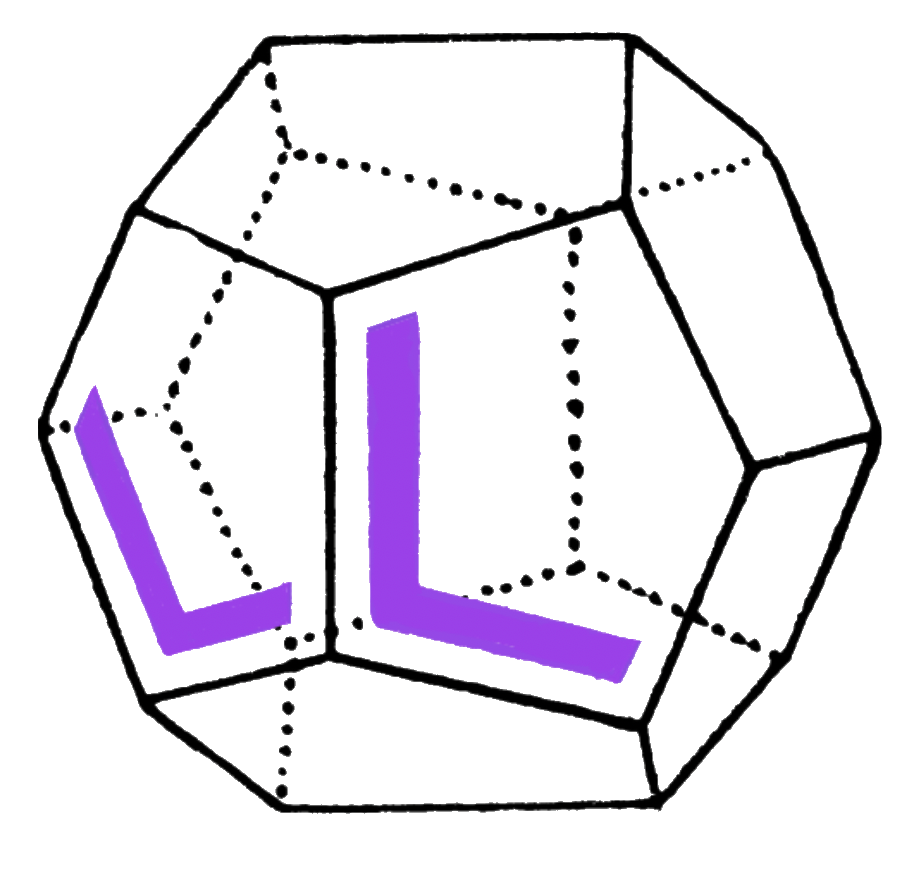
\includegraphics[width=2cm,height=2cm]{ll.png}}

    }}

\AddToShipoutPicture*
  {\put(470,737){

    \href{http://www.linearlibrary.net/CategoryTheory.pdf}{\texttt{.pdf file}}\\

  }}

\AddToShipoutPicture*
  {\put(470,752){
    \href{https://github.com/linlib/CategoryTheory/tree/main}{\texttt{.tex file}}\\

  }}

\AddToShipoutPicture*
  {\put(470,767){
    \href{http://www.linearlibrary.net/CategoryTheory.py}{\texttt{.py file}}

  }}

\AddToShipoutPicture*
  {\put(470,737){

    \href{http://www.linearlibrary.net/CategoryTheory.pdf}{\texttt{.pdf file}}\\

  }}

\AddToShipoutPicture*
  {\put(415,752){
    \href{https://github.com/linlib/CategoryTheory/tree/main}{\texttt{.java file}}\\

  }}

\AddToShipoutPicture*
  {\put(415,767){
    \href{http://www.linearlibrary.net/CategoryTheory.py}{\texttt{.js file}}

  }}

\AddToShipoutPicture*
  {\put(415,737){
    \href{https://github.com/linlib/CategoryTheory/tree/main}{\texttt{.cpp file}}

  }}

\AddToShipoutPicture*
  {\put(415,722){
    \href{https://github.com/linlib/CategoryTheory/tree/main}{\texttt{.c file}}

  }}

\pagecolor{white}

\ \\
\ \\


\thispagestyle{empty} 

\AddToShipoutPicture*
    {\put(540,720){

    \href{http://www.linearlibrary.net}{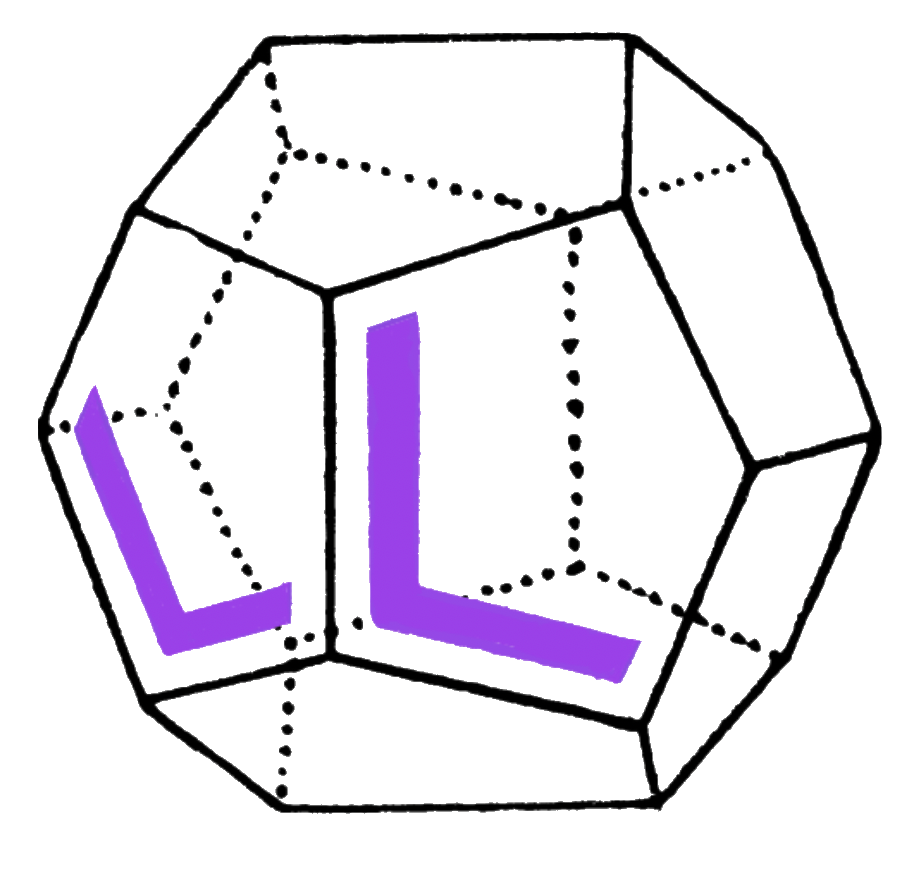
\includegraphics[width=2cm,height=2cm]{ll.png}}

    }}

\AddToShipoutPicture*
  {\put(470,767){
    \href{https://github.com/linlib/ThreeWhiteheadTheorems/StringDiagramGenerator.py}{\texttt{.py file}}
  }}

\AddToShipoutPicture*
  {\put(470,752){
    \href{https://github.com/linlib/ThreeWhiteheadTheorems/ThreeWhiteheadTheorems.tex}{\texttt{.tex file}}\\

  }}


\AddToShipoutPicture*
  {\put(470,737){

    \href{http://linearlibrary.net/ThreeWhiteheadTheorems/October19th.pdf}{\texttt{.pdf file}}\\

  }}

  \AddToShipoutPicture*
  {\put(470,722){
    \href{https://github.com/linlib/ThreeWhiteheadTheorems/ThreeWhiteheadTheorems.lean}{\texttt{.lean file}}

  }}

\ \\

%LEAN: 
\begin{center}
  \begin{tcolorbox}[width=6.5in,colback={white},coltitle=white]
  \begin{center}
  \ \\
  \scalebox{2.3}{\texttt{Internal Universes}}
  \ \\
  \end{center}
  \end{tcolorbox}
  \end{center}
  \ \\

{\footnotesize
\begin{center}
\scalebox{1.1}{
\begin{tabular}{|| l | l || l | l ||} 
\hline
$\texttt{∞\_(∞-Cat)}$   &  $\texttt{D(∞\_(∞-Cat))}$  & $\texttt{∞\_(∞-Cat)⁄C}$    & $\texttt{D(∞\_(∞-Cat)⁄C)}$\\
\hline
$\texttt{∞\_(∞-Grpd)}$  &  $\texttt{D(∞\_(∞-Grpd))}$  & $\texttt{∞\_(∞-Grpd)⁄G}$    & $\texttt{D(∞\_(∞-Grpd)⁄G)}$ \\
 \hline
$\texttt{∞\_(∞-Grpd₀)}$ &  $\texttt{D(∞\_(∞-Grpd₀))}$  & $\texttt{∞\_(∞-Grpd₀)⁄G₀}$  & $\texttt{D(∞\_(∞-Grpd₀)⁄G₀)}$ \\
 \hline
\end{tabular}}
\end{center}}
  
%LEAN: 
\begin{center}
\begin{tcolorbox}[width=2in,colback={white},coltitle=white]
\begin{center}
\scalebox{1.5}{E. Dean Young}
\end{center}
\end{tcolorbox}
\end{center}

\newpage


\thispagestyle{empty}


\newpage
\section{Introduction}

\iffalse
"completion"
coeq ⨿ γⁿ⁺¹ × [γⁿ⁺¹,X] ⇉ ⨿ γⁿ × [γⁿ,X]
\fi



\newpage
\section{Unicode}

Here is a list of the unicode characters I will use:

{\footnotesize
\begin{center}
\begin{tabular}{|| l || l || l || l ||} 
\hline
$\texttt{Symbol}$ & $\texttt{Unicode}$ & \texttt{VSCode shortcut} & $\texttt{Use}$\\
\hline
\hline
\multicolumn{4}{||c||}{\texttt{Lean's Kernel}} \\
\hline
\hline
× & 2A2F & \backslash\texttt{times} & Product of types\\
\hline
→ & 2192 & \backslash\texttt{rightarrow}  & Hom of types\\
\hline
⟨,⟩ & 27E8,27E9 & \backslash\texttt{langle},\backslash\texttt{rangle}  & Product term introduction\\
\hline
↦ & 21A6 &\backslash\texttt{mapsto}  & Hom term introduction\\
\hline
∧ & 2227 &\backslash\texttt{wedge}  & Conjunction \\
\hline
∨ & 2228 &\backslash\texttt{vee}  & Disjunction \\
\hline
∀ & 2200 &\backslash\texttt{forall}  & Universal quantification \\
\hline
∃ & 2203 &\backslash\texttt{exists}  & Existential quantification\\
\hline
¬ & 00AC &\backslash\texttt{neg}  & Negation\\
\hline
\hline
\multicolumn{4}{||c||}{\texttt{Variables and Constants}} \\
\hline
\hline
ᵃ,ᵇ,ᶜ,...,ᶻ & 1D52,1D56 &\iffalse\backslash{}^{$\wedge$}\texttt{a},{\backslash{}}^{$\wedge$}\texttt{b},\backslash{}^{$\wedge$}\texttt{c},...\backslash{}^{$\wedge$}\texttt{z}\fi  & Variables and constants \\
\hline
⁰,¹,²,³,⁴,⁵,⁶,⁷,⁸,⁹ & 1D52,1D56 & \iffalse\backslash\wedge\texttt{0},\backslash{}^{$\wedge$}\texttt{1},\backslash{}^{$\wedge$}\texttt{2},...,\backslash{}^{$\wedge$}\texttt{9}\fi  & Variables and constants \\
\hline
⁻ & 207B & \iffalse\backslash\wedge\texttt{-},\fi  & Variables and constants \\
\hline
₀,₁,₂,₃,₄,₅,₆,₇,₈,₉ & 2080 - 2089 & \backslash\texttt{0}-\backslash\texttt{9} & Variables and constants\\
\hline
𝔸,...,ℤ & 1D538 & \backslash\texttt{bbA},...,\backslash\texttt{bbZ} &  Variables and constants \\
\hline
𝕒,...,𝕫 & 1D552 & \backslash\texttt{bba},...,\backslash\texttt{bbz} & Variables and constants \\
\hline
\iffalse 𝐀,...,𝐙 & 1D41A & \backslash\texttt{bfA},...,\backslash\texttt{bfZ} & Variables and constants \\
\hline
𝐚,...,𝐳 & 1D41A & \backslash\texttt{bfa},...,\backslash\texttt{bfz} & Variables and constants \\
\hline \fi
\texttt{α}-\texttt{ω},\texttt{A}-\texttt{Ω} & 03B1-03C9 & & Variables and constants\\
\hline
\hline
\multicolumn{4}{||c||}{\texttt{Categories and Bicategories}} \\
\hline
\hline
 𝟙 & 1D7D9 & \backslash\texttt{b1}  & The identity morphism\\
\hline
 ≫ & 2218 & & Composition\\
\hline
   &  &  & Composition\\
\hline
   &  &  & Composition\\
\hline
 \multicolumn{4}{||c||}{\texttt{Adjunctions}} \\
\hline
\hline\iffalse
⇄ & 21C4 & \backslash\texttt{rightleftarrows}  & Adjunctions \\
\hline
⇆ & 21C6 & \backslash\texttt{leftrightarrows}  & Adjunctions \\
\hline\fi
𛲔 & 1BC94 &  & Right adjoints\\
\hline
ॱ & 0971 &  & Left adjoints \\
\hline
⊣ & 22A3 & \backslash\texttt{dashv}  & The condition that two functors are adjoint \\
\hline
\hline
\multicolumn{4}{||c||}{\texttt{Monads and Comonads}} \\
\hline
\hline
?,¿ & 003F, 00BF & ?,\backslash\texttt{?}  & The corresponding (co)monad of an adjunction\\
\hline
!,¡ & 0021, 00A1 & !, \backslash\texttt{!}  & The (co)-Eilenberg-(co)-Moore adjunction \\
\hline
ꜝ,ꜞ & A71D, A71E &  & The (co)AdjMon maps\\
\hline
\hline
\multicolumn{4}{||c||}{\texttt{Miscellaneous}} \\
\hline
\hline
\iffalse ∼ & 223C & \backslash\texttt{sim} & Homotopies \\
\hline\fi
≃ & 2243 & \backslash\texttt{equiv}  & Equivalences \\
\hline
≅ & 2245 & \backslash\texttt{cong}   & Isomorphisms \\
\hline
⊥ & 22A5 & \backslash\texttt{bot}    & The overobject classifier \\
\hline
∞ & 221E & \backslash\texttt{infty}  & Infinity categories and infinity groupoids\\ 
 \hline
\end{tabular}
\end{center}}

Of these, the characters $\texttt{ꜝ,ꜞ,𛲔}$ and $\texttt{ॱ}$ do not have VSCode shortcuts, and so I provide alternatives for them. Possibly they will have to be changed if this work assimilates into a larger project.\\

It is not possible to copy the from the pdf to the clipboard while preserving the integrity of the code. To see the official Lean 4 file please click the link on the top right of the front page or \href{https://github.com/linlib/CategoryTheory/tree/main}{this}.



%LEAN: 
\begin{center}
\begin{tcolorbox}[width=5in,colback={white},title={\begin{center}\texttt{Lean \thelcounter} \addtocounter{lcounter}{1}  \end{center}},colbacktitle=Blue,coltitle=black]
\begin{minted}[breaklines, escapeinside=||]{lean}


import Mathlib.CategoryTheory.Bicategory.Basic
import Mathlib.CategoryTheory.Types 
import Mathlib.CategoryTheory.DiscreteCategory
import Mathlib.Combinatorics.Quiver.Basic
import Mathlib.CategoryTheory.Category.Init
import Aesop
import Init
import Mathlib.CategoryTheory.DiscreteCategory
import Mathlib.CategoryTheory.Bicategory.Strict
import Mathlib.CategoryTheory.ConcreteCategory.Bundled
import Mathlib.CategoryTheory.Functor.Basic
import Init.Core
import Mathlib.CategoryTheory.Category.Cat

import TheWhiteheadTheorem

-- #check 
-- #

\end{minted}
\end{tcolorbox}
\end{center}


\newpage
\begin{center}

\pagecolor{white}
\color{black}




\end{center}

\thispagestyle{empty}




\newpage
\pagecolor{white}
\color{black}
\ \\
\ \\
\thispagestyle{empty}
\begin{center}
Copyright\ \textcopyright \ June 2023 Elliot Dean Young.\ All rights reserved.\\
\end{center}
\large %%%%%%%% HERE IS THE large LARGE size textsize set text size
\newpage 
\ \\
\ \\
\ \\
\ \\
\ \\
\ \\
\ \\
\ \\
\ \\
\ \\
\ \\
\thispagestyle{empty}
 
\newpage
\section{Contents}

{
\footnotesize
\begin{longtable}{|| l || l ||} 
\hline
\multicolumn{1}{||c||}{$\texttt{Section}$} & \multicolumn{1}{|c||}{$\texttt{Description}$} \\
\hline
\hline
Unfinished & \\
\hline
Contents & \\
\hline
Unicode & \\
\hline
Introduction & \\
\hline \hline
\multicolumn{2}{||c||}{\texttt{PART I: } Internal Universes} \\
\hline \hline
\multicolumn{2}{||c||}{\texttt{Chapter 1: } ∞\_(∞-Grpd₀)} \\
\hline \hline
χ⃗𛲔 & \\
\hline 
χ⃗ॱ &  \\
\hline
D(χ⃗𛲔) &  \\
\hline
D(χ⃗ॱ) &  \\
\hline
D(∞$\_$(∞-Grpd₋₁)⁄-) &  \\
\hline
D([-ᵒᵖ,∞$\_$(∞-Grpd₋₁)]) &  \\
\hline
D(∞\_(∞-Grpd₋₁)⁄-) ≃ D([-ᵒᵖ,∞\_(∞-Grpd₋₁)]) &  \\
\hline \hline
\multicolumn{2}{||c||}{\texttt{Chapter 2: } ∞\_(∞-Grpd)} \\
\hline \hline
χ⃡𛲔 & \\
\hline
χ⃡ॱ & \\
\hline
D(χ⃡𛲔) & \\
\hline
D(χ⃡ॱ) & \\
\hline
D(∞\_(∞-Grpd)⁄-) & \\
\hline
\iffalse D([-ᵒᵖ,∞\_(∞-Grpd)]) \fi & \\
\hline
\iffalse D(∞\_(∞-Grpd)⁄-) ≃ D([-ᵒᵖ,∞\_(∞-Grpd)]) \fi & \\
\hline \hline
\multicolumn{2}{||c||}{\texttt{Chapter 3: } ∞\_(∞-Cat)} \\
\hline \hline
χ𛲔 & \\
\hline
χॱ & \\
\hline
D(χ𛲔) & \\
\hline
D(χॱ) & \\
\hline
D(∞\_(∞-Cat)⁄-) & \\
\hline
D([-ᵒᵖ,∞\_(∞-Cat)]) & \\
\hline
D(∞\_(∞-Cat)⁄-) ≃ D([-ᵒᵖ,∞\_(∞-Cat)]) & \\
\hline \hline
\multicolumn{2}{||c||}{\texttt{PART II: } Internal Universes} \\
\hline \hline
\multicolumn{2}{||c||}{\texttt{Chapter 4: } Monadicity, D(∞-Grpd₀), and D(∞-Grpd₀⁄X₀) ⇄ D(∞-Grpd₀⁄Y₀)} \\
\hline \hline
 & \\
\hline
 & \\
\hline \hline
\multicolumn{2}{||c||}{\texttt{Chapter 5: } Monadicity, D(∞-Grpd), and D(∞-Grpd⁄X) ⇄ D(∞-Grpd⁄Y)} \\
\hline \hline
 & \\
\hline
 & \\
\hline \hline
\multicolumn{2}{||c||}{\texttt{Chapter 6: } Monadicity, D(∞-Cat), and D(∞-Cat⁄C) ⇄ D(∞-Cat⁄D)} \\
\hline \hline
 & \\
\hline
 & \\
\hline
\end{longtable}
}




\part{Constructing Three Internal Universes}


\chapter{∞\_(∞-Grpd₀)}



\chapter{∞\_(∞-Grpd)}



\chapter{∞\_(∞-Cat)}




\part{Monadicity}


\chapter{Monadicity, D(∞-Grpd₀), and D(∞-Grpd₀⁄X₀) ⇄ D(∞-Grpd₀⁄Y₀)}



\chapter{Monadicity, D(∞-Grpd), and D(∞-Grpd⁄X) ⇄ D(∞-Grpd⁄Y)}



\chapter{Monadicity, D(∞-Cat), and D(∞-Cat⁄C) ⇄ D(∞-Cat⁄D)}





\part{Kan Extensions}
















\newpage 
\ \\
\ \\
\ \\
\ \\
\ \\
\ \\
%LEAN: 
\begin{center}
\begin{tcolorbox}[width=5in,colback={white},title={\begin{center}\texttt{About the Author} \addtocounter{lcounter}{1}  \end{center}},colbacktitle=Yellow,coltitle=black]
Dean Young is a graduate student at New York University, where he studies mathematics. \\

\begin{center}
\iffalse 
\includegraphics[width=7.5cm,height=5cm]{about.jpg}\fi 
\end{center}
\end{tcolorbox}
\end{center}
\newpage
\ \\
\thispagestyle{empty}
\pagecolor{Yellow}



\end{document}







































